\documentclass[a4paper,11pt]{report}

%%%%%%%%%%%%%%%%%%%%%%%%%%%%%%%%%
% PACKAGE IMPORTS
%%%%%%%%%%%%%%%%%%%%%%%%%%%%%%%%%
\usepackage[tmargin=2cm,rmargin=1in,lmargin=1in,margin=0.85in,bmargin=2cm,footskip=.2in]{geometry}
\usepackage[none]{hyphenat}
\usepackage{amsmath,amsfonts,amsthm,amssymb,mathtools}
\allowdisplaybreaks
\usepackage{undertilde}
\usepackage{xfrac}
\usepackage[makeroom]{cancel}
\usepackage{mathtools}
\usepackage{bookmark}
\usepackage{enumitem}
\usepackage{kbordermatrix}
\renewcommand{\kbldelim}{(} % Change left delimiter to (
\renewcommand{\kbrdelim}{)} % Change right delimiter to )
\usepackage{hyperref,theoremref}
\hypersetup{
	pdftitle={Assignment},
	colorlinks=true, linkcolor=doc!90,
	bookmarksnumbered=true,
	bookmarksopen=true
}
\usepackage[most,many,breakable]{tcolorbox}
\usepackage{xcolor}
\usepackage{varwidth}
\usepackage{varwidth}
\usepackage{etoolbox}
%\usepackage{authblk}
\usepackage{nameref}
\usepackage{multicol,array}
\usepackage{tikz-cd}
\usepackage[ruled,vlined,linesnumbered]{algorithm2e}
\usepackage{comment} % enables the use of multi-line comments (\ifx \fi) 
\usepackage{import}
\usepackage{xifthen}
\usepackage{pdfpages}
\usepackage{svg}
\usepackage{transparent}
\usepackage{pgfplots}
\pgfplotsset{compat=1.18}
\usetikzlibrary{calc}
\usetikzlibrary{graphs}
\usetikzlibrary{graphs.standard}
% \usetikzlibrary{graphdrawing}

\newcommand\mycommfont[1]{\footnotesize\ttfamily\textcolor{blue}{#1}}
\SetCommentSty{mycommfont}
\newcommand{\incfig}[1]{%
    \def\svgwidth{\columnwidth}
    \import{./figures/}{#1.pdf_tex}
}


\usepackage{tikzsymbols}
% \renewcommand\qedsymbol{$\Laughey$}

\definecolor{commentgreen}{RGB}{2,112,10}
%%
%% Julia definition (c) 2014 Jubobs
%%
\lstdefinelanguage{Julia}%
  {morekeywords={abstract,break,case,catch,const,continue,do,else,elseif,%
      end,export,false,for,function,immutable,import,importall,if,in,%
      macro,module,otherwise,quote,return,switch,true,try,type,typealias,%
      using,while},%
   sensitive=true,%
   alsoother={$},%
   morecomment=[l]\#,%
   morecomment=[n]{\#=}{=\#},%
   morestring=[s]{"}{"},%
   morestring=[m]{'}{'},%
}[keywords,comments,strings]%

\lstset{%
    language        	= Julia,
    basicstyle      	= \ttfamily,
    keywordstyle    	= \bfseries\color{blue},
    stringstyle     	= \color{magenta},
    commentstyle    	= \color{commentgreen},
    showstringspaces	= false,
		numbers						= left,
		tabsize						= 4,
}

\definecolor{stringyellow}{RGB}{227, 78, 48}
%% 
%% Shamelessly stolen from Vivi on Stackoverflow
%% https://tex.stackexchange.com/questions/75116/what-can-i-use-to-typeset-matlab-code-in-my-document
%%
\lstset{language=Matlab,%
    %basicstyle=\color{red},
    breaklines=true,%
    morekeywords={matlab2tikz},
		morekeywords={subtitle}
    keywordstyle=\color{blue},%
    morekeywords=[2]{1}, keywordstyle=[2]{\color{black}},
    identifierstyle=\color{black},%
    stringstyle=\color{stringyellow},
    commentstyle=\color{commentgreen},%
    showstringspaces=false,%without this there will be a symbol in the places where there is a space
    numbers=left,%
		firstnumber=1,
    % numberstyle={\tiny \color{black}},% size of the numbers
    % numbersep=9pt, % this defines how far the numbers are from the text
    emph=[1]{for,end,break},emphstyle=[1]\color{red}, %some words to emphasise
    %emph=[2]{word1,word2}, emphstyle=[2]{style},    
}

%% 
%% Shamelessly stolen from egreg on Stackoverflow
%% https://tex.stackexchange.com/questions/280681/how-to-have-multiple-lines-of-intertext-within-align-environment
%%
\newlength{\normalparindent}
\AtBeginDocument{\setlength{\normalparindent}{\parindent}}
\newcommand{\longintertext}[1]{%
  \intertext{%
    \parbox{\linewidth}{%
      \setlength{\parindent}{\normalparindent}
      \noindent#1%
    }%
  }%
}

%\usepackage{import}
%\usepackage{xifthen}
%\usepackage{pdfpages}
%\usepackage{transparent}

%%%%%%%%%%%%%%%%%%%%%%%%%%%%%%
% SELF MADE COLORS
%%%%%%%%%%%%%%%%%%%%%%%%%%%%%%
\definecolor{myg}{RGB}{56, 140, 70}
\definecolor{myb}{RGB}{45, 111, 177}
\definecolor{myr}{RGB}{199, 68, 64}
\definecolor{mytheorembg}{HTML}{F2F2F9}
\definecolor{mytheoremfr}{HTML}{00007B}
\definecolor{mylenmabg}{HTML}{FFFAF8}
\definecolor{mylenmafr}{HTML}{983b0f}
\definecolor{mypropbg}{HTML}{f2fbfc}
\definecolor{mypropfr}{HTML}{191971}
\definecolor{myexamplebg}{HTML}{F2FBF8}
\definecolor{myexamplefr}{HTML}{88D6D1}
\definecolor{myexampleti}{HTML}{2A7F7F}
\definecolor{mydefinitbg}{HTML}{E5E5FF}
\definecolor{mydefinitfr}{HTML}{3F3FA3}
\definecolor{notesgreen}{RGB}{0,162,0}
\definecolor{myp}{RGB}{197, 92, 212}
\definecolor{mygr}{HTML}{2C3338}
\definecolor{myred}{RGB}{127,0,0}
\definecolor{myyellow}{RGB}{169,121,69}
\definecolor{myexercisebg}{HTML}{F2FBF8}
\definecolor{myexercisefg}{HTML}{88D6D1}

%%%%%%%%%%%%%%%%%%%%%%%%%%%%
% TCOLORBOX SETUPS
%%%%%%%%%%%%%%%%%%%%%%%%%%%%
\setlength{\parindent}{0pt}

%================================
% THEOREM BOX
%================================
\tcbuselibrary{theorems,skins,hooks}
\newtcbtheorem[number within=section]{Theorem}{Theorem}
{%
	enhanced,
	breakable,
	colback = mytheorembg,
	frame hidden,
	boxrule = 0sp,
	borderline west = {2pt}{0pt}{mytheoremfr},
	sharp corners,
	detach title,
	before upper = \tcbtitle\par\smallskip,
	coltitle = mytheoremfr,
	fonttitle = \bfseries\sffamily,
	description font = \mdseries,
	separator sign none,
	segmentation style={solid, mytheoremfr},
}
{th}

\tcbuselibrary{theorems,skins,hooks}
\newtcbtheorem[number within=chapter]{theorem}{Theorem}
{%
	enhanced,
	breakable,
	colback = mytheorembg,
	frame hidden,
	boxrule = 0sp,
	borderline west = {2pt}{0pt}{mytheoremfr},
	sharp corners,
	detach title,
	before upper = \tcbtitle\par\smallskip,
	coltitle = mytheoremfr,
	fonttitle = \bfseries\sffamily,
	description font = \mdseries,
	separator sign none,
	segmentation style={solid, mytheoremfr},
}
{th}


\tcbuselibrary{theorems,skins,hooks}
\newtcolorbox{Theoremcon}
{%
	enhanced
	,breakable
	,colback = mytheorembg
	,frame hidden
	,boxrule = 0sp
	,borderline west = {2pt}{0pt}{mytheoremfr}
	,sharp corners
	,description font = \mdseries
	,separator sign none
}

%================================
% Corollery
%================================
\tcbuselibrary{theorems,skins,hooks}
\newtcbtheorem[number within=section]{Corollary}{Corollary}
{%
	enhanced
	,breakable
	,colback = myp!10
	,frame hidden
	,boxrule = 0sp
	,borderline west = {2pt}{0pt}{myp!85!black}
	,sharp corners
	,detach title
	,before upper = \tcbtitle\par\smallskip
	,coltitle = myp!85!black
	,fonttitle = \bfseries\sffamily
	,description font = \mdseries
	,separator sign none
	,segmentation style={solid, myp!85!black}
}
{th}
\tcbuselibrary{theorems,skins,hooks}
\newtcbtheorem[number within=chapter]{corollary}{Corollary}
{%
	enhanced
	,breakable
	,colback = myp!10
	,frame hidden
	,boxrule = 0sp
	,borderline west = {2pt}{0pt}{myp!85!black}
	,sharp corners
	,detach title
	,before upper = \tcbtitle\par\smallskip
	,coltitle = myp!85!black
	,fonttitle = \bfseries\sffamily
	,description font = \mdseries
	,separator sign none
	,segmentation style={solid, myp!85!black}
}
{th}

%================================
% LENMA
%================================
\tcbuselibrary{theorems,skins,hooks}
\newtcbtheorem[number within=section]{Lenma}{Lenma}
{%
	enhanced,
	breakable,
	colback = mylenmabg,
	frame hidden,
	boxrule = 0sp,
	borderline west = {2pt}{0pt}{mylenmafr},
	sharp corners,
	detach title,
	before upper = \tcbtitle\par\smallskip,
	coltitle = mylenmafr,
	fonttitle = \bfseries\sffamily,
	description font = \mdseries,
	separator sign none,
	segmentation style={solid, mylenmafr},
}
{th}

\tcbuselibrary{theorems,skins,hooks}
\newtcbtheorem[number within=chapter]{lenma}{Lenma}
{%
	enhanced,
	breakable,
	colback = mylenmabg,
	frame hidden,
	boxrule = 0sp,
	borderline west = {2pt}{0pt}{mylenmafr},
	sharp corners,
	detach title,
	before upper = \tcbtitle\par\smallskip,
	coltitle = mylenmafr,
	fonttitle = \bfseries\sffamily,
	description font = \mdseries,
	separator sign none,
	segmentation style={solid, mylenmafr},
}
{th}

%================================
% PROPOSITION
%================================
\tcbuselibrary{theorems,skins,hooks}
\newtcbtheorem[number within=section]{Prop}{Proposition}
{%
	enhanced,
	breakable,
	colback = mypropbg,
	frame hidden,
	boxrule = 0sp,
	borderline west = {2pt}{0pt}{mypropfr},
	sharp corners,
	detach title,
	before upper = \tcbtitle\par\smallskip,
	coltitle = mypropfr,
	fonttitle = \bfseries\sffamily,
	description font = \mdseries,
	separator sign none,
	segmentation style={solid, mypropfr},
}
{th}

\tcbuselibrary{theorems,skins,hooks}
\newtcbtheorem[number within=chapter]{prop}{Proposition}
{%
	enhanced,
	breakable,
	colback = mypropbg,
	frame hidden,
	boxrule = 0sp,
	borderline west = {2pt}{0pt}{mypropfr},
	sharp corners,
	detach title,
	before upper = \tcbtitle\par\smallskip,
	coltitle = mypropfr,
	fonttitle = \bfseries\sffamily,
	description font = \mdseries,
	separator sign none,
	segmentation style={solid, mypropfr},
}
{th}

%================================
% CLAIM
%================================
\tcbuselibrary{theorems,skins,hooks}
\newtcbtheorem[number within=section]{claim}{Claim}
{%
	enhanced
	,breakable
	,colback = myg!10
	,frame hidden
	,boxrule = 0sp
	,borderline west = {2pt}{0pt}{myg}
	,sharp corners
	,detach title
	,before upper = \tcbtitle\par\smallskip
	,coltitle = myg!85!black
	,fonttitle = \bfseries\sffamily
	,description font = \mdseries
	,separator sign none
	,segmentation style={solid, myg!85!black}
}
{th}

%================================
% Exercise
%================================
\tcbuselibrary{theorems,skins,hooks}
\newtcbtheorem[number within=section]{Exercise}{Exercise}
{%
	enhanced,
	breakable,
	colback = myexercisebg,
	frame hidden,
	boxrule = 0sp,
	borderline west = {2pt}{0pt}{myexercisefg},
	sharp corners,
	detach title,
	before upper = \tcbtitle\par\smallskip,
	coltitle = myexercisefg,
	fonttitle = \bfseries\sffamily,
	description font = \mdseries,
	separator sign none,
	segmentation style={solid, myexercisefg},
}
{th}

\tcbuselibrary{theorems,skins,hooks}
\newtcbtheorem[number within=chapter]{exercise}{Exercise}
{%
	enhanced,
	breakable,
	colback = myexercisebg,
	frame hidden,
	boxrule = 0sp,
	borderline west = {2pt}{0pt}{myexercisefg},
	sharp corners,
	detach title,
	before upper = \tcbtitle\par\smallskip,
	coltitle = myexercisefg,
	fonttitle = \bfseries\sffamily,
	description font = \mdseries,
	separator sign none,
	segmentation style={solid, myexercisefg},
}
{th}

%================================
% EXAMPLE BOX
%================================
\newtcbtheorem[number within=section]{Example}{Example}
{%
	colback = myexamplebg
	,breakable
	,colframe = myexamplefr
	,coltitle = myexampleti
	,boxrule = 1pt
	,sharp corners
	,detach title
	,before upper=\tcbtitle\par\smallskip
	,fonttitle = \bfseries
	,description font = \mdseries
	,separator sign none
	,description delimiters parenthesis
}
{ex}

\newtcbtheorem[number within=chapter]{example}{Example}
{%
	colback = myexamplebg
	,breakable
	,colframe = myexamplefr
	,coltitle = myexampleti
	,boxrule = 1pt
	,sharp corners
	,detach title
	,before upper=\tcbtitle\par\smallskip
	,fonttitle = \bfseries
	,description font = \mdseries
	,separator sign none
	,description delimiters parenthesis
}
{ex}

%================================
% DEFINITION BOX
%================================
\newtcbtheorem[number within=section]{Definition}{Definition}{enhanced,
	before skip=2mm,after skip=2mm, colback=red!5,colframe=red!80!black,boxrule=0.5mm,
	attach boxed title to top left={xshift=1cm,yshift*=1mm-\tcboxedtitleheight}, varwidth boxed title*=-3cm,
	boxed title style={frame code={
					\path[fill=tcbcolback]
					([yshift=-1mm,xshift=-1mm]frame.north west)
					arc[start angle=0,end angle=180,radius=1mm]
					([yshift=-1mm,xshift=1mm]frame.north east)
					arc[start angle=180,end angle=0,radius=1mm];
					\path[left color=tcbcolback!60!black,right color=tcbcolback!60!black,
						middle color=tcbcolback!80!black]
					([xshift=-2mm]frame.north west) -- ([xshift=2mm]frame.north east)
					[rounded corners=1mm]-- ([xshift=1mm,yshift=-1mm]frame.north east)
					-- (frame.south east) -- (frame.south west)
					-- ([xshift=-1mm,yshift=-1mm]frame.north west)
					[sharp corners]-- cycle;
				},interior engine=empty,
		},
	fonttitle=\bfseries,
	title={#2},#1}{def}
\newtcbtheorem[number within=chapter]{definition}{Definition}{enhanced,
	before skip=2mm,after skip=2mm, colback=red!5,colframe=red!80!black,boxrule=0.5mm,
	attach boxed title to top left={xshift=1cm,yshift*=1mm-\tcboxedtitleheight}, varwidth boxed title*=-3cm,
	boxed title style={frame code={
					\path[fill=tcbcolback]
					([yshift=-1mm,xshift=-1mm]frame.north west)
					arc[start angle=0,end angle=180,radius=1mm]
					([yshift=-1mm,xshift=1mm]frame.north east)
					arc[start angle=180,end angle=0,radius=1mm];
					\path[left color=tcbcolback!60!black,right color=tcbcolback!60!black,
						middle color=tcbcolback!80!black]
					([xshift=-2mm]frame.north west) -- ([xshift=2mm]frame.north east)
					[rounded corners=1mm]-- ([xshift=1mm,yshift=-1mm]frame.north east)
					-- (frame.south east) -- (frame.south west)
					-- ([xshift=-1mm,yshift=-1mm]frame.north west)
					[sharp corners]-- cycle;
				},interior engine=empty,
		},
	fonttitle=\bfseries,
	title={#2},#1}{def}

%================================
% Solution BOX
%================================
\makeatletter
\newtcbtheorem{question}{Question}{enhanced,
	breakable,
	colback=white,
	colframe=myb!80!black,
	attach boxed title to top left={yshift*=-\tcboxedtitleheight},
	fonttitle=\bfseries,
	title={#2},
	boxed title size=title,
	boxed title style={%
			sharp corners,
			rounded corners=northwest,
			colback=tcbcolframe,
			boxrule=0pt,
		},
	underlay boxed title={%
			\path[fill=tcbcolframe] (title.south west)--(title.south east)
			to[out=0, in=180] ([xshift=5mm]title.east)--
			(title.center-|frame.east)
			[rounded corners=\kvtcb@arc] |-
			(frame.north) -| cycle;
		},
	#1
}{def}
\makeatother

%================================
% SOLUTION BOX
%================================
\makeatletter
\newtcolorbox{solution}{enhanced,
	breakable,
	colback=white,
	colframe=myg!80!black,
	attach boxed title to top left={yshift*=-\tcboxedtitleheight},
	title=Solution,
	boxed title size=title,
	boxed title style={%
			sharp corners,
			rounded corners=northwest,
			colback=tcbcolframe,
			boxrule=0pt,
		},
	underlay boxed title={%
			\path[fill=tcbcolframe] (title.south west)--(title.south east)
			to[out=0, in=180] ([xshift=5mm]title.east)--
			(title.center-|frame.east)
			[rounded corners=\kvtcb@arc] |-
			(frame.north) -| cycle;
		},
}
\makeatother

%================================
% Question BOX
%================================
\makeatletter
\newtcbtheorem{qstion}{Question}{enhanced,
	breakable,
	colback=white,
	colframe=mygr,
	attach boxed title to top left={yshift*=-\tcboxedtitleheight},
	fonttitle=\bfseries,
	title={#2},
	boxed title size=title,
	boxed title style={%
			sharp corners,
			rounded corners=northwest,
			colback=tcbcolframe,
			boxrule=0pt,
		},
	underlay boxed title={%
			\path[fill=tcbcolframe] (title.south west)--(title.south east)
			to[out=0, in=180] ([xshift=5mm]title.east)--
			(title.center-|frame.east)
			[rounded corners=\kvtcb@arc] |-
			(frame.north) -| cycle;
		},
	#1
}{def}
\makeatother

\newtcbtheorem[number within=chapter]{wconc}{Wrong Concept}{
	breakable,
	enhanced,
	colback=white,
	colframe=myr,
	arc=0pt,
	outer arc=0pt,
	fonttitle=\bfseries\sffamily\large,
	colbacktitle=myr,
	attach boxed title to top left={},
	boxed title style={
			enhanced,
			skin=enhancedfirst jigsaw,
			arc=3pt,
			bottom=0pt,
			interior style={fill=myr}
		},
	#1
}{def}

%================================
% NOTE BOX
%================================
\usetikzlibrary{arrows,calc,shadows.blur}
\tcbuselibrary{skins}
\newtcolorbox{note}[1][]{%
	enhanced jigsaw,
	colback=gray!20!white,%
	colframe=gray!80!black,
	size=small,
	boxrule=1pt,
	title=\textbf{Note:-},
	halign title=flush center,
	coltitle=black,
	breakable,
	drop shadow=black!50!white,
	attach boxed title to top left={xshift=1cm,yshift=-\tcboxedtitleheight/2,yshifttext=-\tcboxedtitleheight/2},
	minipage boxed title=1.5cm,
	boxed title style={%
			colback=white,
			size=fbox,
			boxrule=1pt,
			boxsep=2pt,
			underlay={%
					\coordinate (dotA) at ($(interior.west) + (-0.5pt,0)$);
					\coordinate (dotB) at ($(interior.east) + (0.5pt,0)$);
					\begin{scope}
						\clip (interior.north west) rectangle ([xshift=3ex]interior.east);
						\filldraw [white, blur shadow={shadow opacity=60, shadow yshift=-.75ex}, rounded corners=2pt] (interior.north west) rectangle (interior.south east);
					\end{scope}
					\begin{scope}[gray!80!black]
						\fill (dotA) circle (2pt);
						\fill (dotB) circle (2pt);
					\end{scope}
				},
		},
	#1,
}

%%%%%%%%%%%%%%%%%%%%%%%%%%%%%%
% SELF MADE COMMANDS
%%%%%%%%%%%%%%%%%%%%%%%%%%%%%%
\newcommand{\thm}[2]{\begin{Theorem}{#1}{}#2\end{Theorem}}
\newcommand{\cor}[2]{\begin{Corollary}{#1}{}#2\end{Corollary}}
\newcommand{\mlenma}[2]{\begin{Lenma}{#1}{}#2\end{Lenma}}
\newcommand{\mprop}[2]{\begin{Prop}{#1}{}#2\end{Prop}}
\newcommand{\clm}[3]{\begin{claim}{#1}{#2}#3\end{claim}}
\newcommand{\wc}[2]{\begin{wconc}{#1}{}\setlength{\parindent}{1cm}#2\end{wconc}}
\newcommand{\thmcon}[1]{\begin{Theoremcon}{#1}\end{Theoremcon}}
\newcommand{\ex}[2]{\begin{Example}{#1}{}#2\end{Example}}
\newcommand{\dfn}[2]{\begin{Definition}[colbacktitle=red!75!black]{#1}{}#2\end{Definition}}
\newcommand{\dfnc}[2]{\begin{definition}[colbacktitle=red!75!black]{#1}{}#2\end{definition}}
\newcommand{\qs}[2]{\begin{question}{#1}{}#2\end{question}}
\newcommand{\pf}[2]{\begin{myproof}[#1]#2\end{myproof}}
\newcommand{\nt}[1]{\begin{note}#1\end{note}}

\newcommand*\circled[1]{\tikz[baseline=(char.base)]{
		\node[shape=circle,draw,inner sep=1pt] (char) {#1};}}
\newcommand\getcurrentref[1]{%
	\ifnumequal{\value{#1}}{0}
	{??}
	{\the\value{#1}}%
}
\newcommand{\getCurrentSectionNumber}{\getcurrentref{section}}
\newenvironment{myproof}[1][\proofname]{%
	\proof[\bfseries #1: ]%
}{\endproof}

\newcommand{\mclm}[2]{\begin{myclaim}[#1]#2\end{myclaim}}
\newenvironment{myclaim}[1][\claimname]{\proof[\bfseries #1: ]}{}

\newcounter{mylabelcounter}

\makeatletter
\newcommand{\setword}[2]{%
	\phantomsection
	#1\def\@currentlabel{\unexpanded{#1}}\label{#2}%
}
\makeatother

\tikzset{
	symbol/.style={
			draw=none,
			every to/.append style={
					edge node={node [sloped, allow upside down, auto=false]{$#1$}}}
		}
}

% deliminators
\DeclarePairedDelimiter{\abs}{\lvert}{\rvert}
\DeclarePairedDelimiter{\norm}{\lVert}{\rVert}

\DeclarePairedDelimiter{\ceil}{\lceil}{\rceil}
\DeclarePairedDelimiter{\floor}{\lfloor}{\rfloor}
\DeclarePairedDelimiter{\round}{\lfloor}{\rceil}

\newsavebox\diffdbox
\newcommand{\slantedromand}{{\mathpalette\makesl{d}}}
\newcommand{\makesl}[2]{%
\begingroup
\sbox{\diffdbox}{$\mathsurround=0pt#1\mathrm{#2}$}%
\pdfsave
\pdfsetmatrix{1 0 0.2 1}%
\rlap{\usebox{\diffdbox}}%
\pdfrestore
\hskip\wd\diffdbox
\endgroup
}
\newcommand{\dd}[1][]{\ensuremath{\mathop{}\!\ifstrempty{#1}{%
\slantedromand\@ifnextchar^{\hspace{0.2ex}}{\hspace{0.1ex}}}%
{\slantedromand\hspace{0.2ex}^{#1}}}}
\ProvideDocumentCommand\dv{o m g}{%
  \ensuremath{%
    \IfValueTF{#3}{%
      \IfNoValueTF{#1}{%
        \frac{\dd #2}{\dd #3}%
      }{%
        \frac{\dd^{#1} #2}{\dd #3^{#1}}%
      }%
    }{%
      \IfNoValueTF{#1}{%
        \frac{\dd}{\dd #2}%
      }{%
        \frac{\dd^{#1}}{\dd #2^{#1}}%
      }%
    }%
  }%
}
\providecommand*{\pdv}[3][]{\frac{\partial^{#1}#2}{\partial#3^{#1}}}
%  - others
\DeclareMathOperator{\Lap}{\mathcal{L}}
\DeclareMathOperator{\Var}{Var} % varience
\DeclareMathOperator{\Cov}{Cov} % covarience
\DeclareMathOperator{\E}{E} % expected

% Since the amsthm package isn't loaded

% I dot not prefer the slanted \leq ;P
% % I prefer the slanted \leq
% \let\oldleq\leq % save them in case they're every wanted
% \let\oldgeq\geq
% \renewcommand{\leq}{\leqslant}
% \renewcommand{\geq}{\geqslant}

% % redefine matrix env to allow for alignment, use r as default
% \renewcommand*\env@matrix[1][r]{\hskip -\arraycolsep
%     \let\@ifnextchar\new@ifnextchar
%     \array{*\c@MaxMatrixCols #1}}

%\usepackage{framed}
%\usepackage{titletoc}
%\usepackage{etoolbox}
%\usepackage{lmodern}

%\patchcmd{\tableofcontents}{\contentsname}{\sffamily\contentsname}{}{}

%\renewenvironment{leftbar}
%{\def\FrameCommand{\hspace{6em}%
%		{\color{myyellow}\vrule width 2pt depth 6pt}\hspace{1em}}%
%	\MakeFramed{\parshape 1 0cm \dimexpr\textwidth-6em\relax\FrameRestore}\vskip2pt%
%}
%{\endMakeFramed}

%\titlecontents{chapter}
%[0em]{\vspace*{2\baselineskip}}
%{\parbox{4.5em}{%
%		\hfill\Huge\sffamily\bfseries\color{myred}\thecontentspage}%
%	\vspace*{-2.3\baselineskip}\leftbar\textsc{\small\chaptername~\thecontentslabel}\\\sffamily}
%{}{\endleftbar}
%\titlecontents{section}
%[8.4em]
%{\sffamily\contentslabel{3em}}{}{}
%{\hspace{0.5em}\nobreak\itshape\color{myred}\contentspage}
%\titlecontents{subsection}
%[8.4em]
%{\sffamily\contentslabel{3em}}{}{}  
%{\hspace{0.5em}\nobreak\itshape\color{myred}\contentspage}

%%%%%%%%%%%%%%%%%%%%%%%%%%%%%%%%%%%%%%%%%%%
% TABLE OF CONTENTS
%%%%%%%%%%%%%%%%%%%%%%%%%%%%%%%%%%%%%%%%%%%
\usepackage{tikz}
\definecolor{doc}{RGB}{0,60,110}
\usepackage{titletoc}
\contentsmargin{0cm}
\titlecontents{chapter}[3.7pc]
{\addvspace{30pt}%
	\begin{tikzpicture}[remember picture, overlay]%
		\draw[fill=doc!60,draw=doc!60] (-7,-.1) rectangle (-0.9,.5);%
		\pgftext[left,x=-3.5cm,y=0.2cm]{\color{white}\Large\sc\bfseries Chapter\ \thecontentslabel};%
	\end{tikzpicture}\color{doc!60}\large\sc\bfseries}%
{}
{}
{\;\titlerule\;\large\sc\bfseries Page \thecontentspage
	\begin{tikzpicture}[remember picture, overlay]
		\draw[fill=doc!60,draw=doc!60] (2pt,0) rectangle (4,0.1pt);
	\end{tikzpicture}}%
\titlecontents{section}[3.7pc]
{\addvspace{2pt}}
{\contentslabel[\thecontentslabel]{2pc}}
{}
{\hfill\small \thecontentspage}
[]
\titlecontents*{subsection}[3.7pc]
{\addvspace{-1pt}\small}
{}
{}
{\ --- \small\thecontentspage}
[ \textbullet\ ][]

\makeatletter
\renewcommand{\tableofcontents}{%
	\chapter*{%
	  \vspace*{-20\p@}%
	  \begin{tikzpicture}[remember picture, overlay]%
		  \pgftext[right,x=15cm,y=0.2cm]{\color{doc!60}\Huge\sc\bfseries \contentsname};%
		  \draw[fill=doc!60,draw=doc!60] (13,-.75) rectangle (20,1);%
		  \clip (13,-.75) rectangle (20,1);
		  \pgftext[right,x=15cm,y=0.2cm]{\color{white}\Huge\sc\bfseries \contentsname};%
	  \end{tikzpicture}}%
	\@starttoc{toc}}
\makeatother

\newcommand{\inv}{^{-1}}
\newcommand{\opname}{\operatorname}
\newcommand{\surjto}{\twoheadrightarrow}
% \newcommand{\injto}{\hookrightarrow}
\newcommand{\injto}{\rightarrowtail}
\newcommand{\bijto}{\leftrightarrow}

\newcommand{\liff}{\leftrightarrow}
\newcommand{\notliff}{\mathrel{\ooalign{$\leftrightarrow$\cr\hidewidth$/$\hidewidth}}}
\newcommand{\lthen}{\rightarrow}
\let\varlnot\lnot
\newcommand{\ordsim}{\mathord{\sim}}
\renewcommand{\lnot}{\ordsim}
\newcommand{\lxor}{\oplus}
\newcommand{\lnand}{\barwedge}
\newcommand{\divs}{\mathrel{\mid}}
\newcommand{\ndivs}{\mathrel{\nmid}}
\def\contra{\tikz[baseline, x=0.22em, y=0.22em, line width=0.032em]\draw (0,2.83)--(2.83,0) (0.71,3.54)--(3.54,0.71) (0,0.71)--(2.83,3.54) (0.71,0)--(3.54,2.83);}

\newcommand{\On}{\mathrm{On}} % ordinals
\DeclareMathOperator{\img}{im} % Image
\DeclareMathOperator{\Img}{Im} % Image
\DeclareMathOperator{\coker}{coker} % Cokernel
\DeclareMathOperator{\Coker}{Coker} % Cokernel
\DeclareMathOperator{\Ker}{Ker} % Kernel
\DeclareMathOperator{\rank}{rank}
\DeclareMathOperator{\Spec}{Spec} % spectrum
\DeclareMathOperator{\Tr}{Tr} % trace
\DeclareMathOperator{\pr}{pr} % projection
\DeclareMathOperator{\ext}{ext} % extension
\DeclareMathOperator{\pred}{pred} % predecessor
\DeclareMathOperator{\dom}{dom} % domain
\DeclareMathOperator{\ran}{ran} % range
\DeclareMathOperator{\Hom}{Hom} % homomorphism
\DeclareMathOperator{\Mor}{Mor} % morphisms
\DeclareMathOperator{\End}{End} % endomorphism
\DeclareMathOperator{\Span}{span}
\newcommand{\Mod}{\mathbin{\mathrm{mod}}}

\newcommand{\eps}{\epsilon}
\newcommand{\veps}{\varepsilon}
\newcommand{\ol}{\overline}
\newcommand{\ul}{\underline}
\newcommand{\wt}{\widetilde}
\newcommand{\wh}{\widehat}
\newcommand{\ut}{\utilde}
\newcommand{\unit}[1]{\ut{\hat{#1}}}
\newcommand{\emp}{\varnothing}

\newcommand{\vocab}[1]{\textbf{\color{blue} #1}}
\providecommand{\half}{\frac{1}{2}}
\newcommand{\dang}{\measuredangle} %% Directed angle
\newcommand{\ray}[1]{\overrightarrow{#1}}
\newcommand{\seg}[1]{\overline{#1}}
\newcommand{\arc}[1]{\wideparen{#1}}
\DeclareMathOperator{\cis}{cis}
\DeclareMathOperator*{\lcm}{lcm}
\DeclareMathOperator*{\argmin}{arg min}
\DeclareMathOperator*{\argmax}{arg max}
\newcommand{\cycsum}{\sum_{\mathrm{cyc}}}
\newcommand{\symsum}{\sum_{\mathrm{sym}}}
\newcommand{\cycprod}{\prod_{\mathrm{cyc}}}
\newcommand{\symprod}{\prod_{\mathrm{sym}}}
\newcommand{\parinn}{\setlength{\parindent}{1cm}}
\newcommand{\parinf}{\setlength{\parindent}{0cm}}
% \newcommand{\norm}{\|\cdot\|}
\newcommand{\inorm}{\norm_{\infty}}
\newcommand{\opensets}{\{V_{\alpha}\}_{\alpha\in I}}
\newcommand{\oset}{V_{\alpha}}
\newcommand{\opset}[1]{V_{\alpha_{#1}}}
\newcommand{\lub}{\text{lub}}
\newcommand{\lm}{\lambda}
\newcommand{\uin}{\mathbin{\rotatebox[origin=c]{90}{$\in$}}}
\newcommand{\usubset}{\mathbin{\rotatebox[origin=c]{90}{$\subset$}}}
\newcommand{\lt}{\left}
\newcommand{\rt}{\right}
\newcommand{\bs}[1]{\boldsymbol{#1}}
\newcommand{\exs}{\exists}
\newcommand{\st}{\strut}
\newcommand{\dps}[1]{\displaystyle{#1}}

\newcommand{\sol}{\textbf{\textit{Solution:}} }
\newcommand{\solve}[1]{\textbf{\textit{Solution: }} #1 \qed}
% \newcommand{\proof}{\underline{\textit{proof:}}\\}

\DeclareMathOperator{\sech}{sech}
\DeclareMathOperator{\csch}{csch}
\DeclareMathOperator{\arcsec}{arcsec}
\DeclareMathOperator{\arccsc}{arccsc}
\DeclareMathOperator{\arccot}{arccot}
\DeclareMathOperator{\arsinh}{arsinh}
\DeclareMathOperator{\arcosh}{arcosh}
\DeclareMathOperator{\artanh}{artanh}
\DeclareMathOperator{\arcsch}{arcsch}
\DeclareMathOperator{\arsech}{arsech}
\DeclareMathOperator{\arcoth}{arcoth}

\newcommand{\sinx}{\sin x}          \newcommand{\arcsinx}{\arcsin x}    
\newcommand{\cosx}{\cos x}          \newcommand{\arccosx}{\arccosx}
\newcommand{\tanx}{\tan x}          \newcommand{\arctanx}{\arctan x}
\newcommand{\cscx}{\csc x}          \newcommand{\arccscx}{\arccsc x}
\newcommand{\secx}{\sec x}          \newcommand{\arcsecx}{\arcsec x}
\newcommand{\cotx}{\cot x}          \newcommand{\arccotx}{\arccot x}
\newcommand{\sinhx}{\sinh x}          \newcommand{\arsinhx}{\arsinh x}
\newcommand{\coshx}{\cosh x}          \newcommand{\arcoshx}{\arcosh x}
\newcommand{\tanhx}{\tanh x}          \newcommand{\artanhx}{\artanh x}
\newcommand{\cschx}{\csch x}          \newcommand{\arcschx}{\arcsch x}
\newcommand{\sechx}{\sech x}          \newcommand{\arsechx}{\arsech x}
\newcommand{\cothx}{\coth x}          \newcommand{\arcothx}{\arcoth x}
\newcommand{\lnx}{\ln x}
\newcommand{\expx}{\exp x}

\newcommand{\Theom}{\textbf{Theorem. }}
\newcommand{\Lemma}{\textbf{Lemma. }}
\newcommand{\Corol}{\textbf{Corollary. }}
\newcommand{\Remar}{\textit{Remark. }}
\newcommand{\Defin}[1]{\textbf{Definition} (#1).}
\newcommand{\Claim}{\textbf{Claim. }}
\newcommand{\Propo}{\textbf{Proposition. }}

\newcommand{\lb}{\left(}
\newcommand{\rb}{\right)}
\newcommand{\lbr}{\left\lbrace}
\newcommand{\rbr}{\right\rbrace}
\newcommand{\lsb}{\left[}
\newcommand{\rsb}{\right]}
\newcommand{\bracks}[1]{\lb #1 \rb}
\newcommand{\braces}[1]{\lbr #1 \rbr}
\newcommand{\suchthat}{\medspace\middle|\medspace}
\newcommand{\sqbracks}[1]{\lsb #1 \rsb}
\renewcommand{\abs}[1]{\left| #1 \right|}
\newcommand{\Mag}[1]{\left|\left| #1 \right|\right|}
\renewcommand{\floor}[1]{\left\lfloor #1 \right\rfloor}
\renewcommand{\ceil}[1]{\left\lceil #1 \right\rceil}

\newcommand{\cd}{\cdot}
\newcommand{\tf}{\therefore}
\newcommand{\Let}{\text{Let }}
\newcommand{\Given}{\text{Given }}
% \newcommand{\and}{\text{and }}
\newcommand{\Substitute}{\text{Substitute }}
\newcommand{\Suppose}{\text{Suppose }}
\newcommand{\WeSee}{\text{We see }}
\newcommand{\So}{\text{So }}
\newcommand{\Then}{\text{Then }}
\newcommand{\Choose}{\text{Choose }}
\newcommand{\Take}{\text{Take }}
\newcommand{\false}{\text{False}}
\newcommand{\true}{\text{True}}

\newcommand{\QED}{\hfill \qed}
\newcommand{\CONTRA}{\hfill \contra}

\newcommand{\ihat}{\hat{\imath}}
\newcommand{\jhat}{\hat{\jmath}}
\newcommand{\khat}{\hat{k}}

\newcommand{\grad}{\nabla}
\newcommand{\D}{\Delta}
\renewcommand{\d}{\mathrm{d}}

\renewcommand{\dd}[1]{\frac{\d}{\d #1}}
\newcommand{\dyd}[2][y]{\frac{\d #1}{\d #2}}

\newcommand{\ddx}{\dd{x}}       \newcommand{\ddxsq}{\dyd[^2]{x^2}}
\newcommand{\ddy}{\dd{y}}       \newcommand{\ddysq}{\dyd[^2]{y^2}}
\newcommand{\ddu}{\dd{u}}       \newcommand{\ddusq}{\dyd[^2]{u^2}}
\newcommand{\ddv}{\dd{v}}       \newcommand{\ddvsq}{\dyd[^2]{v^2}}

\newcommand{\dydx}{\dyd{x}}     \newcommand{\dydxsq}{\dyd[^2y]{x^2}}
\newcommand{\dfdx}{\dyd[f]{x}}  \newcommand{\dfdxsq}{\dyd[^2f]{x^2}}
\newcommand{\dudx}{\dyd[u]{x}}  \newcommand{\dudxsq}{\dyd[^2u]{x^2}}
\newcommand{\dvdx}{\dyd[v]{x}}  \newcommand{\dvdxsq}{\dyd[^2v]{x^2}}

\newcommand{\del}[2]{\frac{\partial #1}{\partial #2}}
\newcommand{\Del}[3]{\frac{\partial^{#1} #2}{\partial #3^{#1}}}
\newcommand{\deld}[2]{\dfrac{\partial #1}{\partial #2}}
\newcommand{\Deld}[3]{\dfrac{\partial^{#1} #2}{\partial #3^{#1}}}

\newcommand{\argument}[2]{
  \begin{array}{rll}
    #1
    \cline{2-2}
    \therefore & #2 
  \end{array}
}
% Mathfrak primes
\newcommand{\km}{\mathfrak m}
\newcommand{\kp}{\mathfrak p}
\newcommand{\kq}{\mathfrak q}

%---------------------------------------
% Blackboard Math Fonts :-
%---------------------------------------
\newcommand{\bba}{\mathbb{A}}   \newcommand{\bbn}{\mathbb{N}}
\newcommand{\bbb}{\mathbb{B}}   \newcommand{\bbo}{\mathbb{O}}
\newcommand{\bbc}{\mathbb{C}}   \newcommand{\bbp}{\mathbb{P}}
\newcommand{\bbd}{\mathbb{D}}   \newcommand{\bbq}{\mathbb{Q}}
\newcommand{\bbe}{\mathbb{E}}   \newcommand{\bbr}{\mathbb{R}}
\newcommand{\bbf}{\mathbb{F}}   \newcommand{\bbs}{\mathbb{S}}
\newcommand{\bbg}{\mathbb{G}}   \newcommand{\bbt}{\mathbb{T}}
\newcommand{\bbh}{\mathbb{H}}   \newcommand{\bbu}{\mathbb{U}}
\newcommand{\bbi}{\mathbb{I}}   \newcommand{\bbv}{\mathbb{V}}
\newcommand{\bbj}{\mathbb{J}}   \newcommand{\bbw}{\mathbb{W}}
\newcommand{\bbk}{\mathbb{K}}   \newcommand{\bbx}{\mathbb{X}}
\newcommand{\bbl}{\mathbb{L}}   \newcommand{\bby}{\mathbb{Y}}
\newcommand{\bbm}{\mathbb{M}}   \newcommand{\bbz}{\mathbb{Z}}

%---------------------------------------
% Roman Math Fonts :-
%---------------------------------------
\newcommand{\rma}{\mathrm{A}}   \newcommand{\rmn}{\mathrm{N}}
\newcommand{\rmb}{\mathrm{B}}   \newcommand{\rmo}{\mathrm{O}}
\newcommand{\rmc}{\mathrm{C}}   \newcommand{\rmp}{\mathrm{P}}
\newcommand{\rmd}{\mathrm{D}}   \newcommand{\rmq}{\mathrm{Q}}
\newcommand{\rme}{\mathrm{E}}   \newcommand{\rmr}{\mathrm{R}}
\newcommand{\rmf}{\mathrm{F}}   \newcommand{\rms}{\mathrm{S}}
\newcommand{\rmg}{\mathrm{G}}   \newcommand{\rmt}{\mathrm{T}}
\newcommand{\rmh}{\mathrm{H}}   \newcommand{\rmu}{\mathrm{U}}
\newcommand{\rmi}{\mathrm{I}}   \newcommand{\rmv}{\mathrm{V}}
\newcommand{\rmj}{\mathrm{J}}   \newcommand{\rmw}{\mathrm{W}}
\newcommand{\rmk}{\mathrm{K}}   \newcommand{\rmx}{\mathrm{X}}
\newcommand{\rml}{\mathrm{L}}   \newcommand{\rmy}{\mathrm{Y}}
\newcommand{\rmm}{\mathrm{M}}   \newcommand{\rmz}{\mathrm{Z}}

%---------------------------------------
% Calligraphic Math Fonts :-
%---------------------------------------
\newcommand{\cla}{\mathcal{A}}   \newcommand{\cln}{\mathcal{N}}
\newcommand{\clb}{\mathcal{B}}   \newcommand{\clo}{\mathcal{O}}
\newcommand{\clc}{\mathcal{C}}   \newcommand{\clp}{\mathcal{P}}
\newcommand{\cld}{\mathcal{D}}   \newcommand{\clq}{\mathcal{Q}}
\newcommand{\cle}{\mathcal{E}}   \newcommand{\clr}{\mathcal{R}}
\newcommand{\clf}{\mathcal{F}}   \newcommand{\cls}{\mathcal{S}}
\newcommand{\clg}{\mathcal{G}}   \newcommand{\clt}{\mathcal{T}}
\newcommand{\clh}{\mathcal{H}}   \newcommand{\clu}{\mathcal{U}}
\newcommand{\cli}{\mathcal{I}}   \newcommand{\clv}{\mathcal{V}}
\newcommand{\clj}{\mathcal{J}}   \newcommand{\clw}{\mathcal{W}}
\newcommand{\clk}{\mathcal{K}}   \newcommand{\clx}{\mathcal{X}}
\newcommand{\cll}{\mathcal{L}}   \newcommand{\cly}{\mathcal{Y}}
\newcommand{\calm}{\mathcal{M}}  \newcommand{\clz}{\mathcal{Z}}

%---------------------------------------
% Fraktur  Math Fonts :-
%---------------------------------------
\newcommand{\fka}{\mathfrak{A}}   \newcommand{\fkn}{\mathfrak{N}}
\newcommand{\fkb}{\mathfrak{B}}   \newcommand{\fko}{\mathfrak{O}}
\newcommand{\fkc}{\mathfrak{C}}   \newcommand{\fkp}{\mathfrak{P}}
\newcommand{\fkd}{\mathfrak{D}}   \newcommand{\fkq}{\mathfrak{Q}}
\newcommand{\fke}{\mathfrak{E}}   \newcommand{\fkr}{\mathfrak{R}}
\newcommand{\fkf}{\mathfrak{F}}   \newcommand{\fks}{\mathfrak{S}}
\newcommand{\fkg}{\mathfrak{G}}   \newcommand{\fkt}{\mathfrak{T}}
\newcommand{\fkh}{\mathfrak{H}}   \newcommand{\fku}{\mathfrak{U}}
\newcommand{\fki}{\mathfrak{I}}   \newcommand{\fkv}{\mathfrak{V}}
\newcommand{\fkj}{\mathfrak{J}}   \newcommand{\fkw}{\mathfrak{W}}
\newcommand{\fkk}{\mathfrak{K}}   \newcommand{\fkx}{\mathfrak{X}}
\newcommand{\fkl}{\mathfrak{L}}   \newcommand{\fky}{\mathfrak{Y}}
\newcommand{\fkm}{\mathfrak{M}}   \newcommand{\fkz}{\mathfrak{Z}}


\usepackage{listings}
\usepackage{xcolor}

\definecolor{mathematicaPurple}{rgb}{0.36,0.2,0.5}
\definecolor{mathematicaBlue}{rgb}{0.25,0.35,0.75}
\definecolor{mathematicaGreen}{rgb}{0.0,0.5,0.0}

\lstdefinelanguage{Mathematica}{
  morekeywords={Plot, Solve, Table, Do, Module, If, True, False, Integrate,
    Sum, Limit, Sin, Cos, Exp, Log, Simplify, FullSimplify, Eigenvalues,
    Eigenvectors, D, DSolve, NDSolve, Piecewise},
  sensitive=true,
  morecomment=[l](*),
  morestring=[b]"
}

\lstset{
  language=Mathematica,
  basicstyle=\ttfamily,
  keywordstyle=\color{mathematicaBlue}\bfseries,
  stringstyle=\color{mathematicaGreen},
  commentstyle=\color{mathematicaPurple}\itshape,
  showstringspaces=false,
  breaklines=true,
  columns=flexible,
}

\begin{document}
\begin{center}
{\bf School of Mathematics and Physics, UQ}
\end{center}
\begin{center}
	{\large\bf MATH2100 Applied Mathematical Analysis \\ Semester 2 2025 \\ Problem Set 2} \\ \vspace{1em}
	Michael Kasumagic, 44302669 \\
	Professor Ivana Carrizo Molina \\
	Due 1pm Monday 8 September 2025
\end{center}

\qs{27 marks}{
  The Duffling equation $\ddot{x} - c\dot{x} -4x + x^3 = 0$, with damping constant $c$, models the motin of a mechanical system in a twin-well potential field.
  \begin{enumerate}[label=(\alph*), itemsep=-3pt, topsep=0pt]
    \item Rewrite this second order ODE as a system of first order ODEs.
    \item For $c=0$
    \begin{enumerate}[label=(\roman*), itemsep=-3pt, topsep=0pt]
      \item Find all critical points of the system.
      \item Use linearisation to classify the nature and stability of the critical points
      \item Use the chain rule to solve for the phase curves $y_2 = y_2(y_1)$.
      \item Does the linearised system exhibit qualitatively similar behaviour as the nonlinear?
    \end{enumerate}
    \item (Mathematica) Verify results from part (b)(ii), (iii), and (iv) by plotting a vector field.
    \item For $c=2$
    \begin{enumerate}[label=(\roman*), itemsep=-3pt, topsep=0pt]
      \item Find all critical points of the system.
      \item Calculate the linearised system about each critical point. Classify their nature and stability. If a critical point is a saddle or a node, identify the relevant eigenvalues and eigenvector. If a critical point is a spiral or a centre, describe the direction of rotation, vertical nullclines, and direction field along the axes.
      \item Does the linearised system exhibit qualitatively similar behaviour to the nonlinear?
      \item Sketch a phase portrait for the non-linear system, by hand. Clearly identify each of the critical points and determine the heteroclinic orbit.
    \end{enumerate}
  \end{enumerate}
}
\sol (a)
$$
  \Let y_1 = x,\qquad y_2 = \dot{x}.
$$
$$
  \Then \dot{y}_1 = y_2,\qquad \dot{y}_2 = cy_2 + 4y_1 - y_1^3
$$
Therefore, the second order ODE, as a system of first order ODEs is given by
$$
  \begin{cases}
    \dot{y}_1 = y_2 \\
    \dot{y}_2 = cy_2 + 4y_1 - y_1^3
  \end{cases}
$$

\sol (b)(i) \\
Letting $c=0$, we have
$$
  \begin{cases}
    \dot{y}_1 = y_2 \\
    \dot{y}_2 = 4y_1 - y_1^3
  \end{cases}
$$
Critical points satisfy $\dot{y}_1 = \dot{y}_2 = 0$. \\
If $\dot{y}_1 = 0$ then $y_2 = 0$. \\
If $\dot{y}_2 = 0$ then $0 = 4y_1 - y_1^3 = y_1(4 - y_1^2)$. This means $y_1\in\braces{0, -2, 2}$. \\
Therefore, we have critical points at:
$$
  (0, 0),\qquad (-2,0),\qquad (2,0)
$$

\sol (b)(ii) \\
We find the Jacobian of the system,
$$
  J(y_1,y_2) = \begin{pmatrix} \del{\dot{y}_1}{y_1} & \del{\dot{y}_1}{y_2} \\ \del{\dot{y}_2}{y_1} & \del{\dot{y}_2}{y_2} \end{pmatrix} = \begin{pmatrix} \del{}{y_1}y_2 & \del{}{y_2}y_2 \\ \del{}{y_1}(4y_1 - y_1^3) & \del{}{y_2}(4y_1 - y_1^3) \end{pmatrix} = \begin{pmatrix} 0 & 1 \\ 4 - 3y_1^2 & 0 \end{pmatrix}
$$
Now, we can substitute our 3 critical points:
$$
  J(0,0) = \begin{pmatrix} 0 & 1 \\ 4 & 0 \end{pmatrix},\quad \lm^2 - 4 = 0 \implies \lm = \pm 2.
$$
Real eigenvalues with opposite sign $\implies$ the critical point is an unstable saddle point, along eigenvectors $(1,2)^\rmt$ for $\lm=2$ and $(1,-2)^\rmt$ for $\lm=-2$.
$$
  J(2,0) = \begin{pmatrix} 0 & 1 \\ -8 & 0 \end{pmatrix},\quad \lm^2 + 8 = 0 \implies \lm=\pm2\sqrt{2}i
$$
Complex eigenvalues $\implies$ stable centre of the linearised system. Rotation is clockwise.
$$
  J(-2,0) = \begin{pmatrix} 0 & 1 \\ -8 & 0 \end{pmatrix},\quad \lm^2 + 8 = 0 \implies \lm=\pm2\sqrt{2}i
$$
Exact same nature and stability as previous. \\

\sol (b)(iii) \\
For the phase curve $y_2 = y_2(y_1)$, we note
$$
  \dyd[y_2]{y_1} = \frac{\dot{y}_2}{\dot{y}_1} = \frac{4y_1 - y_1^3}{y_2}.
$$
We can collect terms,
$$
 \dyd[y_2]{y_1} = \frac{4y_1 - y_1^3}{y_2} \iff y_2\d y_2 = \bracks{4y_1 - y_1^3}\d y_1.
$$
Let's now integrate both sides:
$$
 \int y_2\d y_2 = \int \bracks{4y_1 - y_1^3}\d y_1 \iff \frac{1}{2}y_2^2 = 2y_1^2 - \frac{1}{4}y_1^4 + C_1.
$$
That is to say,
$$
  y_2^2 = 4y_1^2 - \frac{1}{2}y_1^4 + C
$$

\sol(b)(iv) \\
The linearised phase plane is qualitatively similar to the nonlinear system near each critical points: a saddle at the origin and centers at $(2,0)$ and $(-2,0)$. However we must be cautious because linearisation is a local tool and the global features (like how trajectories join up across wells) is not determined by the linear model alone. \\

\clearpage
\sol(c) \\
\begin{figure}[h!]
  \begin{center}
    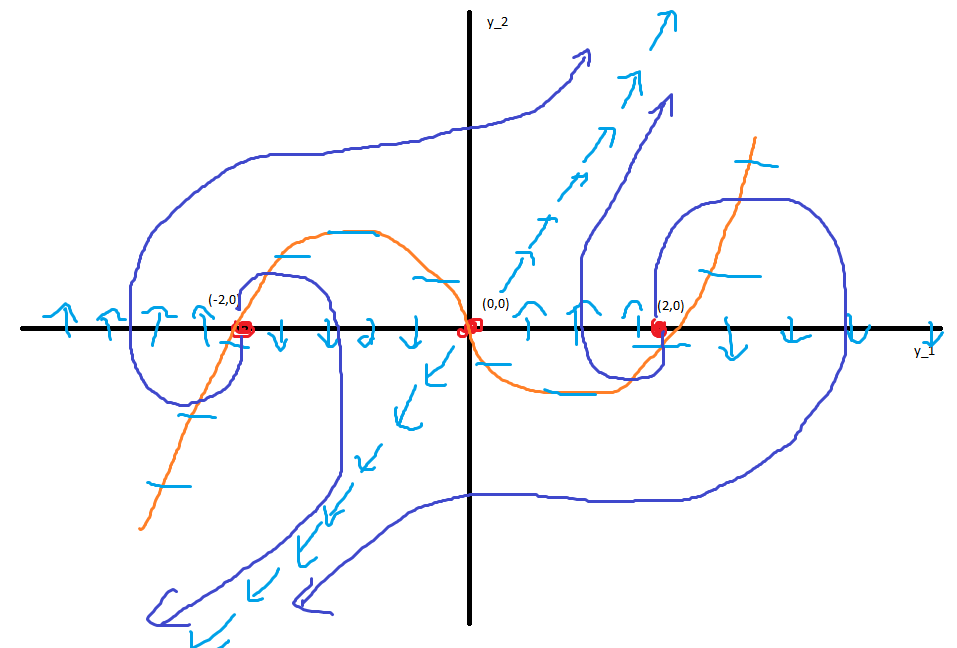
\includegraphics[width=5.5in]{Q1c.png}
    \caption{HAND DRAWN (*in paint). Note the critical points in red, the nullclines in light blue, and the stability/directionality of the spirals highlighed in darkerblue.}
  \end{center}
\end{figure}

\newpage
\sol(d)(i) \\
Letting $c=2$, we have
$$
  \begin{cases}
    \dot{y}_1 = y_2 \\
    \dot{y}_2 = 2y_2 + 4y_1 - y_1^3
  \end{cases}
$$
Critical points satisfy $\dot{y}_1 = \dot{y}_2 = 0$. \\
If $\dot{y}_1 = 0$ then $y_2 = 0$. \\
If $\dot{y}_2 = 0$ then $0 = 2y_2 + 4y_1 - y_1^3 = (4 - y_1^2)y_1 + 2y_2$, but since $y_2=\dot{y}_1=0$ at a critical point, we can simplify this to $0=(4-y_1^2)y_1 \implies y_1\in{0,-2,2}$. \\
Therefore, we get the same critical points as when $c=0$, namely,
$$
  (0, 0),\qquad (-2,0),\qquad (2,0)
$$

\sol (d)(ii) \\
The Jacobian for $c=2$ is similar as that for $c=0$:
$$
  J(y_1,y_2) = \begin{pmatrix} \del{\dot{y}_1}{y_1} & \del{\dot{y}_1}{y_2} \\ \del{\dot{y}_2}{y_1} & \del{\dot{y}_2}{y_2} \end{pmatrix} = \begin{pmatrix} 0 & 1 \\ 4 - 3y_1^2 & 2 \end{pmatrix}.
$$
Now, we can substitute our 3 critical points:
$$
  J(0,0) = \begin{pmatrix} 0 & 1 \\ 4 & 2 \end{pmatrix} \implies \lm = 1 \pm\sqrt{5}.
$$
One eigenvalue is less than zero $\lm_1 = 1 - \sqrt{5}$, and the other, $\lm_2 = 1 + \sqrt{5}$ is greater than 0. Hence, we have an unstable saddle. The unstable eigenvector is $(1, 1+\sqrt{5})^\rmt$, while the stable eigenvector is $(1, 1-\sqrt{5})$.
$$
  J(-2,0) = \begin{pmatrix} 0 & 1 \\ -8 & 2 \end{pmatrix} \implies \lm = 1\pm\sqrt{7}i
$$
Because we have $\Real\lm=1>0$, we have unstable spirals, spinning clockwise. Further, we have $y_1'=0\iff y_2=0$, hence the gradient on the $y_1$-axis is vertical: a vertical nullclines.
$$
  J(2,0) = \begin{pmatrix} 0 & 1 \\ -8 & 2 \end{pmatrix} \implies \lm = 1\pm\sqrt{7}i
$$
So the analysis is exactly the same as the previous.

\sol(d)(iii) \\
Since all three equilibria are hyperbolic ($\det J(y_1,y_2)\neq0$), the linearised system is equivilent to the nonlinear system, in some neighbourhood around each critical point. Therefore, the types and stability at these critical points between either system are the same.

\newpage
\qs{6 marks}{
  Consider the non-linear system of ODEs
  $$
    \begin{array}{l}
      y_1' = f_1'(y_1,y_2) = -2y_1(3-y_2-y_1) \\
      y_2' = f_2'(y_1,y_2) = y_2(-4+y_1+2y_2)      
    \end{array}
  $$
  \begin{enumerate}[label=(\alph*), itemsep=-3pt, topsep=0pt]
    \item (Mathematica) Find all critical points of the system.
    \item (Mathematica) Calculate the linearised system about each critical point. Classify their type and stability.
    \item (Mathematica) Find the nullcines of the system.
    \item (Mathematica) Sketch a phase portrait for the non-linear system. Clearly identify each critical point and nullcine.
  \end{enumerate}
}
\sol (a)
\begin{lstlisting}[language=Mathematica]
In[1] :=  f1[y1_, y2_] := -2 y1 (3 - y2 - y1);
In[2] :=  f2[y1_, y2_] :=  y2 (-4 + y1 + 2 y2);

In[3] :=  critRules = Solve[{f1[y1, y2] == 0, f2[y1, y2] == 0}, {y1, y2}];
In[4] :=  critPts = ({y1, y2} /. critRules)

Out[4]= {{0,0},{0,2},{2,1},{3,0}} 
\end{lstlisting}

\sol (b)
\begin{lstlisting}[language=Mathematica]
In[1] :=  J = D[{f1[y1, y2], f2[y1, y2]}, {{y1, y2}}]
Out[1]:=  {{2 y1-2 (3-y1-y2),2 y1},{y2,-4+y1+4 y2}}
In[2] :=  Do[
            Module[{pt, A, eigs},
              pt   = critPts[[k]];
              A    = J /. Thread[{y1, y2} -> pt];
              eigs = Eigenvalues[A];
              Print[pt, " -> Eigenvalues: ", eigs];
              ],{k, Length[critPts]}
            ]
[OUTPUT:]
{0,2} -> Eigenvalues: {4,-2}
{2,1} -> Eigenvalues: {3+Sqrt[5],3-Sqrt[5]}
{3,0} -> Eigenvalues: {6,-1}
{0,0} -> Eigenvalues: {-6,-4}
\end{lstlisting}
Therefore, the critical point at 
\begin{itemize}[itemsep=0em]
  \item (0,0) is a stable node (2 real negative eigenvalues)
  \item (0,2) is an unstable saddle (2 real, opposite sign eigenvalues)
  \item (2,1) is an unstable saddle (2 real, opposite sign eigenvalues)
  \item (3,0) is an unstable node (2 real positive eigenvalues)
\end{itemize}

\sol (c)
\begin{lstlisting}
In[1] :=  nullcline1 = Reduce[f1[y1, y2] == 0, {y1, y2}]
In[2] :=  nullcline2 = Reduce[f2[y1, y2] == 0, {y1, y2}]
In[3] :=  {nullcline1, nullcline2}
Out[3]:=  y1==0||y2==3-y1
Out[4]:=  y2==0||y2==2-y1/2 
\end{lstlisting}

\sol(d)
\begin{lstlisting}
In[1] :=  phasePortrait = StreamPlot[
            {f1[y1, y2], f2[y1, y2]},
            {y1, Sequence @@ {-1, 6}}, {y2, Sequence @@ {-1, 4}},
            StreamStyle -> Directive[GrayLevel[0.35], Arrowheads[0.02]],
            StreamPoints -> Fine,
            PlotRange -> All,
            FrameLabel -> (Style[#, 14] & /@ {"y1", "y2"}),
            ImageSize -> 520
          ];
  
In[2] :=  nullcline1 = ContourPlot[
            f1[y1, y2] == 0,
            {y1, Sequence @@ {-1, 6}}, {y2, Sequence @@ {-1, 4}},
            ContourStyle -> {Thick, Red},
            PlotLegends -> Placed[{Style["f1=0", Red]}, {0.85, 0.15}],
            PlotRange -> All
          ];

In[3] :=  nullcline2 = ContourPlot[
            f2[y1, y2] == 0,
            {y1, Sequence @@ {-1, 6}}, {y2, Sequence @@ {-1, 4}},
            ContourStyle -> {Thick, Blue},
            PlotLegends -> Placed[{Style["f2=0", Blue]}, {0.85, 0.08}],
            PlotRange -> All
          ];

In[4] :=  critPtsGraphic = Graphics[{
             {Black, PointSize[0.02], Point[critPts]},
             Table[
               Inset[
                 Style[ToString[pt], 12, Black, Background -> White],
                 pt, {Left, Bottom}, {Automatic, Automatic}
               ],
               {pt, critPts}
             ]
          }];  
In[5] :=  Show[phasePortrait, nullcline1, nullcline2, critPtsGraphic, PlotRange -> All]
Out[5]:=
\end{lstlisting}

\clearpage
\begin{figure}[h!]
  \begin{center}
    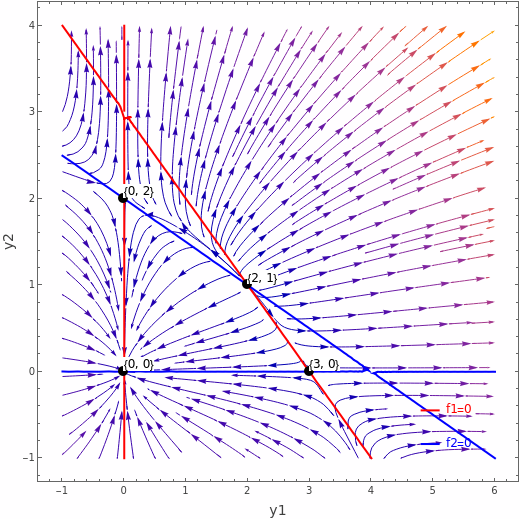
\includegraphics[width=5.5in]{Q2d.png}
    \caption{Final phase space plot for Question 2(d). Note clearly labeled critical points in black, the nullclines in red, and the lines of $0$ or $\infty$ gradient in blue.}
  \end{center}
\end{figure}


\newpage
\qs{7 marks}{
  \begin{enumerate}[label=(\alph*), itemsep=-3pt, topsep=0pt]
    \item (Mathematica) Solve the first order DE
    $$
      \dyd{t} + \frac{2}{t}y(t) = \frac{1}{t^2}
    $$
    \item Consider the IVP 
    $$
      ty'' + 2ty' - 2y = -2,\quad y(0) = 1,\qquad y'(0) = 2.
    $$
    \begin{enumerate}[label=(\roman*), itemsep=-3pt, topsep=0pt]
      \item Apply the Laplace transform to solve for $Y(s)$.
      \item Apply the inverse Laplace transform to $Y(s)$, yielding the solution $y(t)$.
    \end{enumerate}
  \end{enumerate}
}
\sol (a)
\begin{lstlisting}[language=Mathematica]
In[1]   :=  DSolve[a'[t] + (2/t) a[t] == 1/t^2, a[t], t]
Out[1]  :=  {{a[t] -> 1/t + C[1]/t^2}}
\end{lstlisting}
Hence,
$$
  y(t) = \frac{1}{t} + \frac{c}{t^2}
$$

\sol (b)(i) \\
We'll apply the Laplace transform, then solve for $\laplace{y(t)}(s) =: Y(s)$
\begin{align*}
  \laplace{ty'' + 2ty' - 2y}(s) &= \laplace{-2}(s)
  \intertext{First we'll apply linearity,}
  \laplace{ty''}(s) + 2\laplace{ty'}(s) - 2\laplace{y}(s) &= -2\laplace{1}(s)
  \intertext{From the table we have the identities}
  \ignorealign{\laplace{tf(t)} = -\dd{s}\laplace{f(t)}(s) = -\dyd[F]{s} =: -F'(s)} \\
  \ignorealign{\laplace{f^{(n)}(t)}(s) = s^nF(s) - \sum_{i=0}^{n-1} s^if^{(n-i)}(0)} \\
  \intertext{From left to right...}
  \laplace{ty''}(s) &= -\dyd{s} \bracks{s^2Y(s) - sy(0) - y'(0)} \\
    &= -\dyd{s} \bracks{s^2Y(s) - s - 2} \\
    &= -2sY(s) - s^2Y'(s) + 1 + 0  \\
    &= -2sY(s) - s^2Y'(s) + 1  \\
  \laplace{ty'}(s) &= -\dyd{s}\bracks{sY(s) + y(0)} \\
    &= -\dyd{s}\bracks{sY(s) + 1} \\
    &= -Y(s) - sY'(s) \\
  \laplace{y}(s) &= Y \\
  \laplace{1}(s) &= \frac{1}{s} \\
  \intertext{After substituting these values and doing some simplifying, we find that}
  Y'(s^2 + 2s) + Y(2s + 4)  &= 1 + \frac{2}{s}.
  \intertext{Le'ts noe divide through by $s(s+2)$}
  Y' + Y\frac{2s+4}{s(s+2)}  &= \frac{1}{s(s+2)} + \frac{2}{s^2(s+2)} \\
  Y' + Y\frac{2}{s}  &= \frac{s+2}{s^2(s+2)} \\
  Y' + \frac{2}{s} Y  &= \frac{1}{s^2} \\
  \intertext{We note that this is the exact same DE as was given (and solved) in the previous question! This allows us to conclude that}
  Y(s) &= \frac{1}{s} + \frac{C}{s^2}
\end{align*}

\sol(b)(ii)\\
Now we'll apply the inverse Laplace transform to $Y(s)$, hoping to yield the solution, $y(t)$.
\begin{align*}
  \laplace{Y(s)}\inv(t) &= \laplace{\frac{1}{s} + \frac{C}{s^2}}\inv(t) \\
  \intertext{We'll start by applying linearity}
  \laplace{Y(s)}\inv(t) &= \laplace{\frac{1}{s}}\inv(t) + C\laplace{\frac{1}{s^2}}\inv(t) \\
  \intertext{From the table we have}
  \ignorealign{\laplace{1}(s) = \frac{1}{s}\quad\text{and}\quad\laplace{t}(s) = \frac{1}{s^2}}
  \intertext{Applying them, we get}
  \laplace{Y(s)}\inv(t) &= 1 + Ct = y(t)
  \intertext{Applying the initial condition now,}
  y'(t) &= \dd{t}(1 + Ct) \\
    &= C \\
  y'(0) = 2 &\iff C = 2 \\
  \tf y(t) = 1 + 2t.
\end{align*}


\newpage
\qs{10 marks}{
  \begin{enumerate}[label=(\alph*), itemsep=-3pt, topsep=0pt]
    \item Find the Laplace transform of $f(t) = t^5e^{-4t}-7\sin(6t)$.
    \item Let $f(t)$ satisfy the following identity
    $$
      f(t) = (t-1)^2u(t-1) + \int_{0}^{t} f(\tau)\sin(t-\tau)\d\tau.
    $$
    Find the Laplace transform of $f(t)$.
    \item (Mathematica) Use the Laplace-transforms method to solve the IVP
    $$
      \begin{cases}
        y_1'(t) = 3y_1(t) - 4y_2(t),\\
        y_2'(t) = 3y_2(t) - 4y_1(t)
      \end{cases}
    $$
    with initial conditions, $y_1(0)=0$ and $y_2(0)=1$.
    \item (Mathematica) Use \texttt{DSolve} to solve the same IVP, and show the results are equal.
  \end{enumerate}
}
\sol (a) \\
We seek the Laplace transform of $f(t) = t^5e^{-4t}-7\sin(6t)$,
\begin{align*}
  \laplace{f(t)}(s) &= \laplace{t^5e^{-4t}-7\sin(6t)}(s). \\
  \intertext{The Laplace transform is a linear operator, hence}
    &= \laplace{t^5e^{-4t}}(s) + \laplace{-7\sin(6t)}(s) \\
    &= \laplace{t^5e^{-4t}}(s) - 7\laplace{\sin(6t)}(s)
  \intertext{We'll use the table to evaluate these,}
  \ignorealign{\laplace{e^{\alpha t}g(t)}(s) = \laplace{g(t)}(s-\alpha)\qquad \laplace{t^n}(s) = \frac{n!}{s^{n+1}}}
  \intertext{Here, $\alpha=-4,~ g(t)=t^5$, and $n=5$. Therefore}
  \ignorealign{\laplace{t^5e^{-4t}}(s) = \laplace{t^5}(s+4) = \frac{5!}{(s+4)^{s+1}} = \frac{120}{(s+4)^6}}
  \intertext{Now we'll evaluate the other using the table.}
  \laplace{\sin(\alpha t)}(s) &= \frac{\alpha}{s^2 + \alpha^2}
  \intertext{Here, $\alpha=6$, therefore,}
  \ignorealign{\laplace{\sin(6t)}(s) = \frac{6}{s^2 + 6^2} = \frac{6}{s^2 + 36}}
  \intertext{Hence, our transformation comes to}
  \laplace{f(t)}(s) &= \laplace{t^5e^{-4t}}(s) - 7\laplace{\sin(6t)}(s) \\
    &= \frac{120}{(s+4)^6} - 7\cd\frac{6}{s^2 + 36} \\
    &= \frac{120}{(s+4)^6} - \frac{42}{s^2 + 36}
\end{align*}

\newpage
\sol (b) \\
We seek the Laplace transform of 
\begin{align*}
  f(t) &= (t-1)^2u(t-1) + \int_{0}^{t} f(\tau)\sin(t-\tau)\d\tau, \\
  \laplace{f(t)}(s) &= \laplace{(t-1)^2u(t-1) + \int_{0}^{t} f(\tau)\sin(t-\tau)\d\tau}(s).
  \intertext{First, we'll use the linearity of the Laplace transform operator,}
  \laplace{f(t)}(s) &= \laplace{(t-1)^2u(t-1)}(s) + \laplace{\int_{0}^{t} f(\tau)\sin(t-\tau)\d\tau}(s).
  \intertext{Second shifting theorem states}
  \laplace{f(t-k)u(t-k)}(s) &= e^{-ks}\laplace{f(t)}(s).
  \intertext{In our case $k=1$, and $f(t)=t^2$, hence}
  \ignorealign{\laplace{(t-1)^2u(t-1)}(s) = e^{-1s}\laplace{t^2}(s) = e^{-s}\cd\frac{2!}{s^{2+1}} = \frac{2e^{-s}}{s^{3}}}
  \intertext{Convolution theorem states}
  \laplace{\int_{0}^{t} f(\tau)g(t-\tau)\d\tau}(s) &= \laplace{f(t)}(s)\cd\laplace{g(t)}(s).
  \intertext{We have $f(\tau)$ and $g(t)=\sin(t)$. Hence,}
  \laplace{\int_{0}^{t} f(\tau)\sin(t-\tau)\d\tau}(s) &= \laplace{f(t)}(s)\cd\laplace{\sin t}(s) \\
    &= \laplace{f(t)}(s)\cd\frac{1}{s^2+1^2}
  \intertext{Let $F(s) := \laplace{f(t)}(s)$. Hence, we have}
  \laplace{f(t){(s)}} = F(s) &= \frac{2e^{-s}}{s^{3}} + F(s)\cd\frac{1}{s^2+1} \\
  \implies F(s)\bracks{1 - \frac{1}{s^2+1}} &= \frac{2e^{-s}}{s^{3}} \\
  \tf F(s) &= \frac{2e^{-s}}{s^{3}} \div \bracks{1 - \frac{1}{s^2+1}} \\
    &= \frac{2e^{-s}}{s^{3}}\bracks{\frac{s^2+1}{s^2}} \\
  \intertext{Therefore, an arbitrary function defined by the identify}
  f(t) &= (t-1)^2u(t-1) + \int_{0}^{t} f(\tau)\sin(t-\tau)\d\tau
  \intertext{has Laplace transform}
  \laplace{f(t)}(s) &= \frac{2e^{-s}(s^2+1)}{s^{5}}.
\end{align*}

\newpage
\sol (c)(i)
\begin{lstlisting}[language=Mathematica]
In[1]   :=  A = {{3, -4}, {-4, 3}};
            y0 = {0, 1};
            LapY = Inverse[s*IdentityMatrix[2] - A] . y0;
            y = InverseLaplaceTransform[LapY, s, t]
Out[4]  := {-(1/2) Exp[-t] (-1 + Exp[8 t]), 1/2 Exp[-t] (1 + Exp[8 t])}
\end{lstlisting}

First we set the matrix \texttt{A} to the coefficents, as they were given in the question, namely
$$
  \mathbf{Y}'(t) = A\mathbf{Y}(t) \iff \begin{pmatrix} y_1'(t) \\ y_2'(t) \end{pmatrix} = \begin{pmatrix} 3 & -4 \\ -4 & 3 \end{pmatrix} \begin{pmatrix} y_1(t) \\ y_2(t) \end{pmatrix}^\rmt \implies A = \begin{pmatrix} 3 & -4 \\ -4 & 3 \end{pmatrix}.
$$
Next we set a vector to represent the intial condition, \texttt{y0}, by
$$
  \textbf{Y}(0) = \begin{pmatrix} y_1 (0) \\ y_2(0) \end{pmatrix} = \begin{pmatrix} 0 \\ 1 \end{pmatrix}
$$
Applying the Laplace transform to
$$ 
  \mathbf Y'(t)=A\mathbf Y(t)
$$
with $\mathbf Y(0)=\mathbf y_0$ yields
$$
  s\mathbf Y(s)-\mathbf y_0=A\mathbf Y(s),
$$
hence
$$
  (sI-A)\mathbf{Y}(s)=\mathbf y_0\quad \text{and}\quad \mathbf{Y}(s)=(sI-A)^{-1}\mathbf y_0.
$$
The inverse Laplace transform gets us our desired result! \\

\sol (c)(ii)
\begin{lstlisting}[language=Mathematica]
In[1]   :=  eqs = {y1'[t] == 3 y1[t] - 4 y2[t], y2'[t] == 3 y2[t] - 4 y1[t], 
              y1[0] == 0, y2[0] == 1};             
In[2]   :=  solDS = DSolve[eqs, {y1, y2}, t][[1]];
In[3]   :=  solLap = {y1[t] -> -(1/2) Exp[-t] (-1 + Exp[8 t]),
              y2[t] -> 1/2 Exp[-t] (1 + Exp[8 t])};
In[4]   :=  ({y1[t], y2[t]} /. solDS) == ({y1[t], y2[t]} /. solLap)
Out[4]  :=  True
\end{lstlisting}
We set the system of DEs, along with the initial values in the \texttt{eqs} variable. We then solve it numerically and store the first solution it found in \texttt{solDS}. Next we store the Laplace solution from the previous question in \texttt{solLap}. Finally, we compare the solutions, and find that they are equal.

\end{document}